% #######################################
% ########### FILL THESE IN #############
% #######################################
\def\mytitle{CIRCLE ASSIGNMENT}
\def\mykeywords{}
\def\myauthor{SIVA PARVATHI TUNGALA}
\def\contact{tvssn143@gmail.com}
\def\mymodule{ Future Wireless Communication(FWC22089)}
% #######################################
% #### YOU DON'T NEED TO TOUCH BELOW ####
% #######################################
\newcommand{\myvec}[1]{\ensuremath{\begin{pmatrix}#1\end{pmatrix}}}
\let\vec\mathbf
\providecommand{\pr}[1]{\ensuremath{\Pr\left(#1\right)}}
\providecommand{\qfunc}[1]{\ensuremath{Q\left(#1\right)}}
\providecommand{\sbrak}[1]{\ensuremath{{}\left[#1\right]}}
\providecommand{\lsbrak}[1]{\ensuremath{{}\left[#1\right.}}
\providecommand{\rsbrak}[1]{\ensuremath{{}\left.#1\right]}}
\providecommand{\brak}[1]{\ensuremath{\left(#1\right)}}
\providecommand{\lbrak}[1]{\ensuremath{\left(#1\right.}}
\providecommand{\rbrak}[1]{\ensuremath{\left.#1\right)}}
\providecommand{\cbrak}[1]{\ensuremath{\left\{#1\right\}}}
\providecommand{\lcbrak}[1]{\ensuremath{\left\{#1\right.}}
\providecommand{\rcbrak}[1]{\ensuremath{\left.#1\right\}}}
\documentclass[10pt, a4paper]{article}
\usepackage[a4paper,outer=1.5cm,inner=1.5cm,top=1.75cm,bottom=1.5cm]{geometry}
\twocolumn
\usepackage{circuitikz}
\usepackage{amsmath,bm}
\usepackage{amsthm}
\usepackage{mathtools}
\usepackage{amsfonts}
\usepackage{amssymb}
\usepackage{graphicx}
\usepackage{bm}
\newcommand{\bfitDelta}{\bm{\mathit{\Delta}}}

\graphicspath{{./images/}}
%colour our links, remove weird boxes
\usepackage[colorlinks,linkcolor={black},citecolor={blue!80!black},urlcolor={blue!80!black}]{hyperref}
%Stop indentation on new paragraphs
\usepackage[parfill]{parskip}
%% Arial-like font
\usepackage{lmodern}
\renewcommand*\familydefault{\sfdefault}
%Napier logo top right
\usepackage{watermark}
%Lorem Ipusm dolor please don't leave any in you final report ;)
\usepackage{karnaugh-map} 
\usepackage{tabularx}
\usepackage{lipsum}
\usepackage{xcolor}
\usepackage{listings}
%give us the Capital H that we all know and love
\usepackage{float}
%tone down the line spacing after section titles
\usepackage{titlesec}
%Cool maths printing
\usepackage{amsmath}
%PseudoCode
\usepackage{algorithm2e}

\titlespacing{\subsection}{0pt}{\parskip}{-3pt}
\titlespacing{\subsubsection}{0pt}{\parskip}{-\parskip}
\titlespacing{\paragraph}{0pt}{\parskip}{\parskip}
\newcommand{\figuremacro}[5]{
    \begin{figure}[#1]
        \centering
        \includegraphics[width=#5\columnwidth]{#2}
        \caption[#3]{\textbf{#3}#4}
        \label{fig:#2}
    \end{figure}
}


 \lstset{
frame=single, 
breaklines=true,
columns=fullflexible
}
\thiswatermark{\centering \put(1,-110){
\includegraphics[scale=0.05]{iitlogo.jpg}} }
\title{\mytitle}
\author{\myauthor\hspace{1em}\\\contact\\IITH\hspace{0.5em}-\hspace{0.5em}\mymodule}
\date{}
\hypersetup{pdfauthor=\myauthor,pdftitle=\mytitle,pdfkeywords=\mykeywords}
\sloppy
% #######################################
% ########### START FROM HERE ###########
% #######################################
\begin{document}
 \maketitle
 \tableofcontents
 
    
 

 
    
    
    
 
 \Large\section{Problem}
 Q.Let $T_1,T_2$ be two tangents drawn from  (-2,0) onto the circle $C:{x}^2+{y}^2=1$. Determine the circles touching C and having $T_1,T_2$ as their pair of tangents. Further ,find the equations of all possible common tangents to the circles.


\Large\section{Figure}

\begin{figure}[H]
\centering
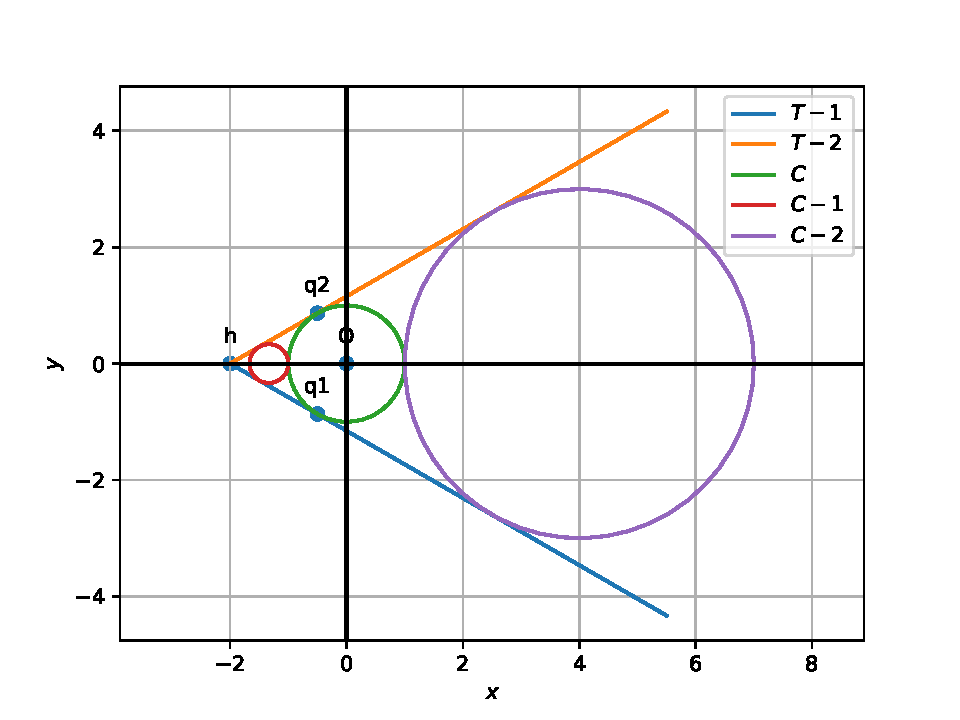
\includegraphics[width=1\columnwidth]{cfig.pdf}
\caption{Labeling}
\label{fig:triangle}
\end{figure}


 \section{Solution}
\raggedright Let, the centre of a circle C\\ be 'u' is  at origin and radius be 'r'. \\
 the equation of the circle is given by
 \begin{align}
  \large \textbf{x}^\top\textbf{Vx} + 2\textbf{u}^\top\textbf{x} +f =0
 \end{align}
\centering
\begin{tabular}{|c |c |}
     \hline % <-- Alignments: 1st column left, 2nd middle and 3rd right, with vertical lines in between
	\large\textbf{Symbol} & \large\textbf{Co-ordinates}  \\
       \hline
	\large \textbf{u} & $\myvec{0\\0}$  \\
        \hline
	 \large \textbf{V} & $\myvec{1&0\\0&1}$\\
       \hline
     \large \textbf{h} & $\myvec{-2\\0}$ \\
        \hline
    \end{tabular}

\raggedright To find the normal vectors at the point of contact , drawn from the eternal point, the normal vectors are given as follows
\begin{align}
\large\boxed{\textbf{q}_{i} = \textbf{V}^{-1}(k_i\textbf{n}_{i}-\textbf{u})}....(i=1,2)
\end{align}
Here,
\begin{align}
\large k_i= \pm\sqrt{\frac{f_0}{\textbf{n}^\top\textbf{V}^{-1}\textbf{n}}}
\end{align} 
\begin{align}
\large f_0=\textbf{u}^\top\textbf{V}^{-1}\textbf{u}-f \\
f=-r^2
\end{align}
\begin{align}
\large  \textbf{S}=(\textbf{Vh+u})(\textbf{Vh+u})^\top\textbf{-}\textbf{V}(\textbf{h}^\top\textbf{Vh}+\textbf{2u}^\top\textbf{h})+f
\end{align}
\begin{align}
\large \textbf{n}_{1}=\textbf{P}\myvec{ \sqrt{|\lambda_1|} \\ \sqrt{|\lambda_2|} } 
\end{align}
\begin{align}
\large \textbf{n}_{2}=\textbf{P}\myvec{ \sqrt{|\lambda_1|} \\ -\sqrt{|\lambda_2|} }
\end{align}

By substituting values in eq(4) we get,
\begin{align}
\large \textbf{S}= \myvec{ 1 &0 \\0 &-3}
\end{align}
The values of eigen values and vectors are by solving we get,\\
$\lambda_1 = 1 $ , $\lambda_2 = -3 $ and \large $\textbf{P}=\myvec{1&0\\0&1}$ \\

\Large from eq(6) and (7), \\
\begin{align}
\textbf{n}_{1}=\myvec{1 \\ \sqrt{3}} \\
\textbf{n}_{2}=\myvec{1 \\ -\sqrt{3}}
\end{align}
To find the equation through a point we have ,
\begin{align}
\textbf{n}^\top(\textsc{x}-\textbf{h})=0
\end{align}
Tangent equation $ T_1 $ and $T_2$ are ,
\begin{align}
\textbf{n}_{1}^\top(\textsc{x}-\textbf{h})=0 \\
\textbf{n}_{2}^\top(\textsc{x}-\textbf{h})=0
\end{align}  

Considering the circles $ C_1 $ and $C_2$ touching C and having $ T_1 $ and $T_2$ are as their pair of tangents. To prove $ T_1 $ and $T_2$  are the common tangents to the circles,let  $\textbf{u}_{1}$ and $\textbf{u}_{2}$ be the centre of circles $ C_1 $ and $C_2$ then \\
\begin{align}
\textbf{u}_{1}=\myvec{-h_1 \\ 0} and \hspace{0.3cm} \textbf{u}_{2}=\myvec{h_2 \\ 0} 
\end{align}
Case(i) : \\
The distance between point $\textbf{u}_{1}$  to the line $ T_1 $ can be taken as, 
\begin{align}
\large d=\frac{|\textbf{n}_{1}^\top\textbf{u}_{1}-c|}{\|\textbf{n}_{1}\|} 
\end{align}
$r_1$ is the radius of circle $C_1$
\begin{align}
r_1=\frac{|\myvec{ 1 & \sqrt{3} }\myvec{-h_1 \\ 0}+2|}{\sqrt{4}} \\
r_1=\frac{h_1+2}{2}
\end{align}
from diagram $r_1$ can be written as,
\begin{align}
r_1=-h_1-1
\end{align}
from eq(16) and (17),
\begin{align}
\textbf{u}_{1}=\myvec{\frac{-4}{3} \\ 0}
\end{align}

Similarly Case(ii) : \\
The distance between point $\textbf{u}_{2}$ to the line $T_1$ is,
\begin{align}
r_2=\frac{h_2+2}{2}
\end{align}
from diagram $r_2$ can be written as,
\begin{align}
r_2=h_2-1
\end{align}
from eq(20) and (21)
\begin{align}
\textbf{u}_{2}=\myvec{4\\0}
\end{align}
Substituting $\textbf{u}_{1}$ and $\textbf{u}_{2}$ in circle equations we get,
\begin{align}
\large\textbf{x}^\top\textbf{Vx} + 2\textbf{u}_{1}^\top\textbf{x} +f =0 \\
\large\textbf{x}^\top\textbf{Vx} + 2\textbf{u}_{2}^\top\textbf{x} +f =0
 \end{align}
Therefore, the all possible common tangents to the circles are x+$\sqrt{3}$y+2=0 and x-$\sqrt{3}$y+2=0.


\section{Software}
  We can get the parallel equation of given equation and the plot of two equtions by executing the following code:
 \vspace{1mm} 
\begin{lstlisting}
https://github.com/sivaparvathi-tungala/fwc_module_1/tree/main/circle
\end{lstlisting}
\end{document}